\chapter*{Notational Conventions and Preliminaries}
\addcontentsline{toc}{chapter}{Notational Conventions and Preliminaries}

\label{ch-not-cons}
\section{Some abbreviations frequently
used throughout this book}

\begin{itemize}
\item
bnet= Bnet= Bayesian Network
\item
CPT = Conditional Probabilities Table,
 same as TPM
\item
DAG = Directed Acyclic Graph
\item
i.i.d.= independent identically 
distributed.
 \item
 RCT= Randomized Controlled Trial,
aka A/B testing.

\item
TPM= Transition Probability Matrix,
same as CPT

\end{itemize}

\section{${\cal N}(!a)$}
$\caln(!a)$ will denote 
a normalization constant that does not depend
on $a$. For example, $P(x)=\caln(!x)e^{-x}$
where $\int_0^\infty dx \;P(x)=1$.

\section{One hot}
A {\bf one hot } vector of zeros and 
ones is a vector with all entries 
zero with
the exception of a single entry which is one.
A {\bf one cold} vector has all entries
equal to one with the exception of  a
single entry which is zero.
For example, if $x^n=(x_0, x_1, \ldots,
x_{n-1})$ and
$x_i=\delta(i,0)$ then $x^n$ is one hot.


\section{Special sets}
Define $\ZZ, \RR, \CC$ to be
 the integers, real numbers
 and complex numbers, respectively. 

For $a<b$, define $I_\ZZ$ 
to be the integers in the 
interval $I$, where 
$I=[a,b],[a,b),(a,b],(a,b)$ 
(i.e, $I$ can be closed or
 open on either side).

$A_{>0}=\{k\in A: k>0\}$ for $A=\ZZ, \RR$.

\section{Kronecker 
delta function}

 For $x,y$ in discrete set $S$, 
\beq
\delta(x,y)=\left\{
\begin{array}{l}
1\;{\rm if}\; x=y
\\
0 \;{\rm if}\; x\neq y
\end{array}
\right.
\eeq

\section{Dirac delta function}
 For $x,y\in\RR$,
\beq
\int^{+\infty}_{-\infty}dx\;\delta(x-y)f(x)=f(y)
\eeq

\section{Indicator function 
(aka Truth function)}
\beq
\indi(\cals)=\left\{
\begin{array}{l}
1\;{\rm if\; \cals\; is\; true} 
\\
0 \;{\rm if \;\cals\; is \;false}
\end{array}
\right.
\eeq
For example, $\delta(x,y)=\indi(x=y)$.

\section{Majority function}
The {\bf majority function}  is defined as follows.

\beq
\begin{array}{ll}
{\tt majority}(L)=&
\text{ most common element of  list $L$}
\\
&\text{(ties resolved by chance)}
\end{array}
\eeq
Note that the majority function
acts on lists, not sets. By definition, 
all elements of a set appear only once in the set.
${\tt majority}(L)$
is usually
used when the elements of
$L$ are categorical (i.e., not real numbers).
When they are real numbers,
it makes more sense to use, instead of 
${\tt majority}(L)$, a simple average
of the elements of $L$.


\section{Underlined letters
 indicate random variables}
Random variables will be indicated by 
underlined letters and their values 
by non-underlined letters.
 Each node of a bnet will be
 labelled by a random variable.
 Thus, $\rvx=x$ means that node 
$\rvx$ is in state $x$.

It is more
conventional to
use an upper
case letter to 
indicate
a random 
variable
and a lower case letter
for its state.
Thus, $X=x$ means that 
random variable
$X$ is in state $x$.
However,
we have
opted
in this
book to
avoid
that notation,
because
we often
want to define
certain lower
case letters 
to be random variables
or, conversely, define certain upper
case letters to 
be non-random variables.

\section{Probability distributions}
 $P_\rvx(x)=P(\rvx=x)=P(x)$ is the probability that random variable $\rvx$ equals $x\in S_\rvx$. $S_\rvx$ is the set of states (i.e., values) that $\rvx$ can assume and $n_\rvx = |S_\rvx|$ is the size (aka cardinality) of that set. Hence, 
\beq
\sum_{x\in S_\rvx}P_\rvx(x)=1
\eeq

\hrule
\beq
P_{\rvx,\rvy}(x,y)=P(\rvx=x, \rvy=y)=P(x,y)
\eeq
\beq
P_{\rvx|\rvy}(x|y)=P(\rvx=x| \rvy=y)=P(x|y)=\frac{P(x,y)}{P(y)}
\eeq



\section{Discretization
of continuous
probability distributions}

The TPM of a node 
of a bnet can be either a discrete or 
a continuous probability distribution. 
To go from continuous to discrete, one 
replaces integrals over states of a node
 by sums over new states, and Dirac delta 
functions by Kronecker delta functions.
 More precisely, consider a function 
$f: [a, b]\rarrow \RR$. Express
 $[a,b]$ as 
a union of
small, disjoint (except for
one point) closed sub-intervals (bins) of
length $\Delta x$.
Name one point
in each bin to be the representative of that bin,
and  let $S_\rvx$ be the
set of all the bin representatives. This is called 
discretization or binning. Then

\beq 
\frac{1}{(b-a)}
\int_{[a,b]} dx \; f(x)\rarrow
\frac{\Delta x}{(b-a)} \sum_{x\in S_\rvx}f(x)
=
\frac{1}{n_\rvx} \sum_{x\in S_\rvx}f(x)
 \;.
\eeq
Both sides of last equation are 1 when $f(x)=1$.
 Furthermore, if $y\in S_\rvx$, then

\beq 
\int_{[a,b]} dx \; \delta(x-y)f(x)=f(y)
\rarrow \sum_{x\in S_\rvx}\delta(x,y)f(x)
=f(y)
\;.
\eeq


\section{Samples, 
i.i.d. variables}
\beq
\vec{x}= (x[0], x[1], x[2] \ldots,
 x[nsam(\vecx)-1])=x[:]
\eeq

 $nsam(\vecx)$ is the number of samples 
 of $\vecx$. 
$\rvx[\sigma]\in S_\rvx$ are
 i.i.d. (independent identically distributed) 
samples with

 \beq
x[\sigma]\sim P_\rvx\;\;({\rm i.e.}\; P_{\ul{x[\sigma]}}=P_\rvx)
\eeq

\beq
P(\rvx=x)=\frac{1}{nsam(\vecx)}\sum_\sigma \indi(x[\sigma]=x)
\eeq 
Hence, for any $f:S_\rvx\rarrow \RR$,
\beq
\sum_x P(\rvx=x)f(x)
=\frac{1}{nsam(\vecx)}\sum_\sigma f(x[\sigma])
\eeq 


If we use two sampled variables, say $\vecx$ and $\vecy$, 
in a given bnet, their number of samples 
$nsam(\vecx)$ and $nsam(\vecy)$ need not be equal.

\hrule
\beq
P(\vecx) = \prod_\sigma P(x[\sigma])
\eeq

\beq
\sum_\vecx = \prod_\sigma\sum_{x[\sigma]}
\eeq

\beq
\partial_\vecx = 
[\partial_{x[0]}, \partial_{x[1]},\partial_{x[2]}, \dots, \partial_{x[nsam(\vecx)-1]}]
\eeq

\hrule
\beqa
P(\vecx)&\approx& [\prod_x P(x)^{P(x)}]^{nsam(\vecx)} \\
&=& e^{nsam(\vecx)\sum_x P(x)\ln P(x)}\\
&=& e^{-nsam(\vecx)H(P_\rvx)}
\eeqa


\section{Normal Distribution}
For $x, \mu, \sigma\in \RR$, $\sigma >0$

\beq 
\caln(x; \mu, \sigma^2)=
\frac{1}{\sigma\sqrt{2\pi}}
e^{-\frac{1}{2}\left(
\frac{x-\mu}{\sigma}\right)^2}
\eeq

\section{Uniform Distribution}
For $a<b$, $x\in [a,b]$

\beq
\calu(x;a,b) =
\frac{1}{b-a}
\eeq

\section{Sigmoid and logit functions}

The sigmoid function sig:$\RR\rarrow [0,1]$
is defined by
\beq
\smoid(x)=
\frac{1}{1+e^{-x}}
\eeq
$\smoid()$ is monotonically
increasing with $\smoid(-\infty)=0$ and $\smoid(+\infty)=1$.

The logit or log-odds function 
logit:$[0,1]\rarrow \RR$ is defined by

\beq
{\rm logit}(p)=\ln\frac{p}{1-p}
\eeq

logit() is the inverse of $\smoid()$:
\beq
{\rm logit}[\smoid(x)]=x
\eeq



\section{Expected Value and Variance}

Given a random variable
 $\rvx$ with states $S_\rvx$ and 
a function $f:S_\rvx\rarrow \RR$, define

\beq
E_\rvx[f(\rvx)]=
E_{x\sim P(x)}[f(x)] = \sum_x P(x) f(x)
\eeq

\beqa
Var_\rvx[f(\rvx)]&=& E_\rvx
\left[(f(\rvx)-E_\rvx[f(\rvx)])^2\right]
\\
&=&
E_\rvx[f(\rvx)^2]-(E_\rvx[f(\rvx)])^2 
\eeqa

\beq
E[\rvx]=E_\rvx[\rvx]
\eeq

\beq
Var[\rvx]=
Var_\rvx[\rvx]
\eeq

\section{Conditional Expected Value}

Given a random variable $\rvx$ with states $S_\rvx$, a random variable $\rvy$ with states $S_\rvy,$ and a function $f:S_\rvx\times S_\rvy\rarrow \RR$, define

\beq
E_{\rvx|\rvy}[f(\rvx, \rvy)]=
\sum_x P(x|\rvy) f(x, \rvy)
\;,
\eeq

\beq
E_{\rvx|\rvy=y}[f(\rvx, y)]=
E_{\rvx|y}[f(\rvx, y)]= \sum_x P(x| y) f(x, y)
\;.
\eeq
Note that

\beqa
E_\rvy[E_{\rvx|\rvy}[f(\rvx, \rvy)]]&=&
\sum_{x,y}P(x|y)P(y)f(x,y)
\\&=&
\sum_{x,y}P(x,y)f(x,y)
\\&=&
E_{\rvx, \rvy}[f(\rvx, \rvy)]
\;.
\eeqa

\section{Law of Total Variance}

\begin{claim}
Suppose $P:S_\rvx\times S_\rvy\rarrow [0,1]$
is a probability distribution.
Suppose $f:S_\rvx\times S_\rvy\rarrow \RR$
 and $f=f(x,y)$. Then
\beq
Var_{\rvx, \rvy}(f)=
E_\rvy[Var_{\rvx|\rvy}(f)]
+
Var_\rvy(E_{\rvx|\rvy}[f])
\;.
\eeq
In particular,
\beq
Var_{\rvx}(x)=
E_\rvy[Var_{\rvx|\rvy}(x)]
+
Var_\rvy(E_{\rvx|\rvy}[x])
\;.
\eeq

\end{claim}
\proof

Let
\beq
A=\sum_y P(y)\left(\sum_x P(x|y)f\right)^2
\;.
\eeq
Then

\beqa
Var_{\rvx, \rvy}(f)&=& \sum_{x,y}P(x,y)f^2 -
\left( \sum_{x,y} P(x,y) f\right)^2
\\
&=&
\left\{
\begin{array}{l}
\sum_{x,y}P(x,y)f^2 
-A
\\
+\left(A-\left( \sum_{x,y} P(x,y) f\right)^2\right)
\end{array}
\right.
\eeqa

\beqa
E_\rvy[Var_{\rvx|\rvy}(f)]
&=&
\sum_y P(y)\left(\sum_x P(x|y)f^2
-
\left(\sum_x P(x|y)f\right)^2
\right)
\\
&=&
\sum_{x,y}P(x,y)f^2 
-A
\eeqa

\beqa
Var_\rvy(E_{\rvx|\rvy}[f])
&=&
\sum_y P(y)
\left(\sum_x P(x|y)f\right)^2
-\left(
\sum_y P(y)\sum_xP(x|y)f
\right)^2
\\
&=&
A-\left( \sum_{x,y} P(x,y) f\right)^2
\eeqa
\qed

\section{Notation
for covariances}
Consider two random variables $\rvx, \rvy$.

\begin{itemize}
\item
Mean value of $\rvx$
\beq
\av{\rvx}=
E_\rvx[\rvx]
\eeq

\item
Signed distance of $\rvx$ to its mean value
\beq
\Delta \rvx = \rvx - \av{\rvx}
\eeq

\item
Covariance of $(\rvx, \rvy)$
\beq
Cov(\rvx, \rvy)=\av{\rvx, \rvy}=
\av{\Delta \rvx \Delta \rvy}
=
\av{\rvx\rvy}-\av{\rvx}\av{\rvy}
\eeq

$\av{\rvx, \rvy}$ is symmetric 
(i.e., $\av{\rvx, \rvy}=\av{\rvy, \rvx}$)
and bilinear (i.e.,
$\av{\sum_i \alp_i\rvx_i, \rvy}
=
\sum_i\alp_i\av{\rvx_i, \rvy}$, where
$\alp_i\in \RR$
are non-random scalars
and $\rvx_i, \rvy\in\RR$ are 
real-valued random
variables.)

\item
Variance of $\rvx$
\beq
Var(\rvx)=\av{\rvx, \rvx}
\eeq

\item
Standard deviation or $\rvx$
\beq
\sigma_\rvx=\sqrt{\av{\rvx, \rvx}}
\eeq

\item
Correlation Coefficient of $(\rvx, \rvy)$
\beq
\rho_{\rvx, \rvy}=
\frac{\av{\rvx, \rvy}}
{\sqrt{\av{\rvx, \rvx}\av{\rvy, \rvy}}}
\eeq
\end{itemize}

\section{Conditional Covariance}
Let $\rvx, \rvy, \rva$
be random variables.
The covariance $Cov(\rvx, \rvy|\rva)$
of $\rvx$ and $\rvy$ 
given $\rva$, is defined
the same
way as $Cov(\rvx, \rvy)$,
except that all
expected values are 
conditioned on $\rva$. 



\beq
Cov(\rvx, \rvy|\rva)=
\av{\rvx, \rvy}_{|\rva}
=
\av{(\rvx-\av{\rvx}_{|\rva})
(\rvy-\av{\rvy}_{|\rva})}_{|\rva}
\eeq
where

\beq
\av{\rvx}_{|\rva}=E_{\rvx|\rva}[\rvx]
\;.
\eeq

\section{Linear regression, Ordinary Least Squares (OLS)}
Wikipedia articles
\begin{enumerate}
\item
Linear Regression (LR)
\begin{itemize}
\item
linear regression, Ref.\cite{wiki-lr}
\item
 simple linear regression, Ref.\cite{wiki-slr}
\item
errors in variable, Ref.\cite{wiki-errors-in-iv}

\end{itemize}
\item
Least squares (LS)
\begin{itemize}
\item
least squares, Ref.\cite{wiki-ls}
\item
ordinary least squares (OLS), Ref.\cite{wiki-ols}
\end{itemize}
\end{enumerate}


In LR, the {\bf dependent variables} 
$y$
equal
a linear combination of some
{\bf independent variables} $x$ 
 plus some external noise variables
$\eps$ called the {\bf residuals}.

Below, we consider two types of LR:

\begin{enumerate}
\item
LR
in which the independent
 variables are non-random.
\item
LR
in which the independent
 variables are random
and i.i.d.
\end{enumerate}

Once one assumes that certain
variables are random, a ``model" (i.e., a bnet)
for the random variables must be 
specified.

For LR of type 2,
there is randomness in $y$ 
coming from the randomness in $x$
and in the residuals.
For LR of type 1,
there  is randomness in $y$
too, but
it comes 
from the residuals
only. 

OLS provides a
cost function which
when minimized, yields LR.
The  term OLS
is often used to refer to LR 
of type 1.

\subsection{LR, assuming
$x_\s$ are non-random}

Let

$\s\in\{0, 1, 2, \ldots, nsam-1\}$ : sample index

$y_\s\in \RR$: dependent variables

$x_{\s j}\in \RR$: independent variables

$\eps_\s\in \RR$: residuals

$\beta_0, \beta_j\in \RR$: 
regression coefficients


\beq
y_\s= \beta_0 +
\sum_{j=1}^n x_{\s j}\beta_j + \eps_\s
\eeq

If we define
\beq
x_{\s 0}=1
\;
\eeq
for all $\s$, then

\beq
y_\s=
\sum_{j=0}^n x_{\s j}\beta_j + \eps_\s
\;.
\eeq
If $y$ and $\eps$ are $nsam\times 1$
 column vectors and $\beta$
is an $(n+1)\times 1$ column vector, 
then can write previous equation in matrix
form as:


\beq
y=X\beta+\eps
\;.
\eeq

Define the {\bf projection matrices}

\beq
\A=X(X^TX)^{-1}X^T
\;,\;\;\V=1-\A
\eeq
A square matrix $M$ 
is symmetric if $M^T=M$
and is idempotent if $M^2=M$.
$\A$ is symmetric
and idempotent 
and so is $\V$.
Note that $\A$ and $\V$ 
also satisfy:  

\beq
\V\A=\A\V=0
\eeq
and

\beq
\A X=X\;,\;\; \V X=0
\;.
\eeq

One has

\beq
\beta=
(X^TX)^{-1}X^T(y-\eps)
\;.
\eeq


Define 

\begin{subequations}
\beq \boxed{
\hat{\beta}=
(X^TX)^{-1}X^Ty=By
\;,
}
\label{eq-beta-nonrandom-lin-reg}
\eeq



\beq
\hat{y}=
X\hat{\beta}= \A y
\;,
\eeq
and

\beq
\hat{\eps}=
y-X\hat{\beta}=
y-\hat{y}=(1-\A)y=\V y
\;.
\eeq
\end{subequations}
$\A$ is sometimes  called the {\bf hat matrix},
because it gives $y$ a hat. 

Given any function $f=f(y,X,\eps)$
and a scalar factor $\xi\in \RR$,
suppose 
$f(\xi y, \xi X, \xi\eps)=\xi^\calo f(y,X,\eps)$.
Then we will say that $f(\cdot)$
is of {\bf order $\calo$ under scaling}.
Note that $\{X, y,\hat{y},\eps,
 \hat{\eps}\}$
are all of order 1 under scaling,
$\{\beta, \hat{\beta}, \A, \V\}$
are all of order 0 under scaling,
and $B$ is of order $-1$ under scaling.
Thus, the estimator variables (i.e, those
with a hat) 
scale the same way as the variables
without a hat that they are estimating. Furthermore,
$\beta$, its estimator $\hat{\beta}$, and
the projection matrices $\A, \V$
are invariant ($\calo=0$) under scaling.



Fig.\ref{fig-y-yhay-ehat}
illustrates that $y$ 
can be expressed as
a sum of 2 estimators:
 


\beq
y= \underbrace{\hat{y}}_{\A y} + 
\underbrace{\hat{\eps}}_{\V y}
\;.
\eeq

\begin{figure}[h!]
$$
\xymatrix{
&&
\\
&&{}
\\
{}\ar[uurr]^{y}
\ar[rr]_{\hat{y}=\A y}
&&{}\ar[uu]_{\hat{\eps}=\V y}
}
$$
\caption{
Decomposition of $y$
into sum of two estimators, $\hat{y}$ and
$\hat{\eps}$.
}
\label{fig-y-yhay-ehat}
\end{figure}



\hrule
\noindent{\bf model dependent results}:

Assume the components of $\eps$ 
are random over $\s$
and

\beq
E_\s[\rveps]=\av{\rveps}=0
\eeq



Assume $X$ and $\beta$ are not random.
This makes $\rvy=X\beta +\rveps$ and $\ul{\hat{\beta}}=
(X^TX)^{-1}X^T\rvy
$
random.
One finds that

\beq
\av{\rvy}=X\beta
\eeq

\begin{subequations}
\beq
\av{\hat{\rvy}}=\A\av{\rvy}=\av{\rvy}
\eeq

\beq
\av{\hat{\rveps}}=\V\av{\rvy}=0
\eeq

\beq
\av{\ul{\hat{\beta}}}=\beta
\eeq


So far, we have
assumed a zero mean value for $\eps$.
Next, assume  
{\bf  ``homoscedasticity" (HS)}, which
means that 

\beq
\av{\rveps, \rveps^T}=\xi^2 I_{nsam}
\eeq
\end{subequations}
where
$\xi\geq 0$,  $nsam=\sum_\s$ and 
$I_{nsam}$ is the
$nsam\times nsam$ identity matrix.
It follows that

\beq
\av{\rvy, \rvy^T}=
\av{\rveps, \rveps^T}=
\xi^2 I_{nsam}
\;,
\eeq

\beq
\av{\hat{\rveps},
\hat{\rveps}^T}=
\V\av{\rvy, \rvy^T}\V^T=\xi^2\V
\label{eq-homo}
\;,
\eeq

\beq
\av{\hat{\rvy},
\hat{\rvy}^T}=
\A\av{\rvy, \rvy^T}\A^T=\xi^2\A
\eeq
and

\beq
\av{\hat{\ul{\beta}},
\hat{\ul{\beta}}^T}=
B\av{\rvy, \rvy^T}B^T=\xi^2 (X^TX)^{-1}
\;.
\eeq

The goodness of fit
for this model
is often measured using  the
{\bf coefficient of determination}
$R^2$. $R^2$  is defined by


\beq
R^2=
\frac{
\norm{\hat{\rvy}-\av{\hat{\rvy}}}^2
}{
\norm{\rvy-\av{\rvy}}^2
}
=
\frac{
\tr\av{\hat{\rvy},
\hat{\rvy}^T}
}{
\tr\av{\rvy,\rvy^T}
}
\eeq
If HS holds, then
$R^2$ reduces to


\beq
R^2 =\frac{\tr\; \A}{nsam}
\;.
\eeq

\subsection{LR, assuming
$x_\s$ are random and i.i.d.}
Let

$\rvy\in\RR$:  true value
of dependent variable

$\hat{\rvy}\in\RR$: estimator
of dependent variable

$\ul{\eps}\in\RR$: residual

$\rvx_j\in \RR$: independent variables

$\beta_0, \beta_j\in\RR$:
regression coefficients

\beq
\hat{\rvy}=
\beta_0 +\sum_{j=1}^n\beta_j \rvx_j
\eeq

\beq
\rvy = \hat{\rvy}+\ul{\eps}
\eeq
Assume 

\beq
\av{\rveps}=0
\eeq
and
\beq
\av{\rvx_j, \ul{\eps}}=0
\eeq
for all $j$.

For $k=1, \ldots, n$,
\beq
\av{\rvx_k, \rvy}
=
\sum_{j=1}^n\beta_j\av{\rvx_k, \rvx_j}
\;.
\eeq
Let $\rvx^n$ and $\beta^n$ be
column vectors.
Then
\beq
\av{\rvx^n, \rvy}=
\av{\rvx^n, (\rvx^n)^T}\beta^n
\;,
\eeq

\beq
\boxed{
\beta^n=
\av{\rvx^n, (\rvx^n)^T}^{-1}
\av{ \rvx^n, \rvy}
\;.}
\label{eq-beta-random-lin-reg}
\eeq

\beq
\beta_0=
\av{\rvy}-(\beta^n)^T \av{\rvx^n}
\eeq

Notice that 
the equations for the regression coefficients
are very similar
for the two cases of $x_\s$-nonrandom
and $x_\s$-random.
In fact, if  we replace bilinears as follows

\beq
X^T y\longrightarrow\av{\rvx^n, \rvy} 
\eeq

\beq
X^T X
\longrightarrow \av{\rvx^n, (\rvx^n)^T}
\eeq
we go from the estimator  
of $\beta$ for one case
to the estimator 
of $\beta$ for the other case:

\beq
\text{
Eq.(\ref{eq-beta-nonrandom-lin-reg})}
\longrightarrow
\text{
Eq.(\ref{eq-beta-random-lin-reg})}
\eeq

Next, we will
write 
 Eq.(\ref{eq-beta-random-lin-reg})
for the special cases
$n=1$ and $n=2$,
where $n$ is the 
number of independent 
variables $\rvx_j$

\begin{enumerate}
\item $n=1$ ($\rvy$ fitted by a line)

\beq
\rvy = \beta_0 + \beta\rvx + \rveps
\eeq

Eq.\ref{eq-beta-random-lin-reg} becomes
\beq
\beta_{\rvy,\rvx}=
\beta=
\frac{\av{\rvy,\rvx}}{\av{\rvx,\rvx}}
\eeq


\item $n=2$ ($\rvy$ fitted by a plane)


\beq
\rvy = \beta_0 + \beta_1 \rvx_1 + \beta_2 \rvx_2 +\rveps
\eeq
Define


\beq 
C_{i,j}=\av{\rvx_i, \rvx_j}
\eeq  
for all $i,j$.
Then Eq.\ref{eq-beta-random-lin-reg}
becomes\footnote{
Recall that if
$
M=
\left[
\begin{array}{cc}
a&b
\\
c&d
\end{array}
\right]
$
then
$
M^{-1}
=
\frac{1}{\det M}
\left[
\begin{array}{cc}
d&-b
\\
-c&a
\end{array}
\right]
$
}


\beqa
\left[
\begin{array}{c}
\beta_1
\\
\beta_2
\end{array}
\right]
&=&
C^{-1}
\left[
\begin{array}{c}
\av{\rvy, \rvx_1}
\\
\av{\rvy, \rvx_2}
\end{array}
\right]
\\
&=&
\frac{1}{\det C}
\left[
\begin{array}{cc}
C_{22}&-C_{12}
\\
-C_{21}&C_{11}
\end{array}
\right]
\left[
\begin{array}{c}
\av{\rvy, \rvx_1}
\\
\av{\rvy, \rvx_2}
\end{array}
\right]
\eeqa  


Hence,
\beq
 \beta_{\rvy,\rvx_1|\rvx_2}=
\beta_1
=
\frac{
C_{22}\av{\rvy, \rvx_1}
-C_{12}\av{\rvy, \rvx_2}
}
{
C_{11}C_{12}-C_{12}^2
}
\label{eq-beta-lr-plane}
\eeq
Eq.(\ref{eq-beta-lr-plane})
 agrees with 
the
value of $\beta_{YX| Z}$ in
Ref.\cite{pearl-lin-reg} 
by Pearl,
if  we replace in Pearl's 
formulae $X\rarrow \rvx_1$,
$Y\rarrow \rvy$, $Z\rarrow \rvx_2$.


\end{enumerate}





\section{Entropy, Kullback-Liebler divergence}

For probabilty distributions $p(x), q(x)$ of $x\in S_\rvx$
\begin{itemize}
\item 
Entropy:
\beq
H(p)=-\sum_x p(x)\ln p(x)\geq 0
\eeq

\item
Kullback-Liebler divergence:

\beq
D_{KL}(p\parallel q)=\sum_{x} p(x)\ln \frac{p(x)}{q(x)}\geq 0
\eeq
\item 
Cross entropy:
\beqa
CE(p\rarrow q) &=& -\sum_x p(x)\ln q(x)\\
&=& H(p) + D_{KL}(p\parallel q)
\eeqa
\end{itemize}

\section{Definition of various
entropies used in Shannon Information Theory}

\begin{itemize}
\item
{\bf (plain) Entropy of $\rvx$}

\beq
H(\rvx) =
-\sum_{x} P(x)\ln P(x)
\eeq
This quantity measures the
spread of $P_\rvx$.
$H(\rvx)\geq 0$
and it vanishes iff $P(x)=\delta(x,x_0)$ (deterministic case)


\item
{\bf Conditional Entropy of $\rvy$ given $\rvx$}

\beqa
H(\rvy|\rvx) &=&
-\sum_{x,y}P(x,y)\ln {P(y|x)}
\\
&=&
H(\rvy,\rvx)-H(\rvx)
\eeqa
This quantity measures  the conditional
 spread
of $\rvy$ given $\rvx$. $H(\rvy|\rvx)\geq 0$.


\item {\bf Mutual Information (MI)
of $\rvx$ and $\rvy$}.

\beqa
H(\rvy:\rvx) &=&
\sum_{x,y} P(x,y) \ln \frac{P(x,y)}{P(x)P(y)}
\\
&=&
H(\rvx) + H(\rvy) - H(\rvy,\rvx)
\eeqa
This quantity measures the correlation
between $\rvx$ and $\rvy$.
$H(\rvy:\rvx)\geq 0$ 
and it vanishes iff
$P(x,y)=P(x)P(y)$.

\item {\bf Conditional Mutual Information 
(CMI)\footnote{CMI
can be read as ``see me".}
of $\rvx$ and $\rvy$
given $\ul{\lam}$}


\beqa
H(\rvy:\rvx|\ul{\lam})
&=&
\sum_{x,y, \lam}P(x,y, \lam) \ln
\frac{P(x,y|\lam)}{P(x|\lam)P(y|\lam)}
\\
&=&
H(\rvx|\ul{\lam}) + H(\rvy|\ul{\lam})
- H(\rvy,\rvx|\ul{\lam})
\eeqa

This
quantity measures the conditional correlation
of $\rvx$ and $\rvy$ given $\ul{\lam}$.
$H(\rvy:\rvx|\ul{\lam})\geq 0$ 
and it vanishes iff
$P(x,y|\lam)=P(x|\lam)P(y|\lam)$.

An interesting special case 
occurs when 
$P(\lam)=\delta(\lam, \lam_0)$ (the
frequentist  case of no $\lam$ prior.)
In that case CMI
reduces to 

\beq
H(\rvy:\rvx|\lam_0)
=
\sum_{x,y}P(x,y|\lam_0) \ln
\frac{P(x,y|\lam_0)}{P(x|\lam_0)P(y|\lam_0)}\geq 0
\eeq



\item {\bf Kullback-Liebler Divergence
from $P_\rvx$ to $P_\rvy$.}

Assume random variables $\rvx$
and $\rvy$
have the same set of states
$S_\rvx=S_\rvy$. Then


\beq
D_{KL}(P_\rvx\parallel P_\rvy)=
\sum_x P_\rvx(x) \ln \frac{P_\rvx(x)}{P_\rvy(x)}
\eeq

This quantity measures a non-symmetric distance
between the probability distributions
$P_\rvx$ and $P_\rvy$. 
$D_{KL}(P_\rvx\parallel P_\rvy)\geq 0$ 
and it equals zero iff $P_\rvx=P_\rvy$.


\end{itemize}

\section{Pearson Chi-Squared Test}

The
{\bf Pearson divergence}
(aka {\bf Pearson Chi-squared test statistic})
for two
probability distributions
$PO(x)$ and $PE(x)$,
where $x\in S_\rvx$,
is defined 
as follows:
\beq
D_{\chi^2}=
\sum_x
\frac{[PO(x)-PE(x)]^2}{PE(x)}
=
\sum_x \frac{PO^2(x)}{PE(x)}-1
\;.
\eeq
Usually $PO$ is the
observed probability distribution and 
$PE$ is the expected, theoretical one.

As the following claim shows,
the Pearson divergence
is closely related to the 
Kullback-Liebler divergence.

 
\begin{claim}
If $\left|\frac{PO(x)}{PE(x)}-1\right|<<1$
for all $x\in S_\rvx$, then

\beq
D_{KL}(PO\parallel PE)\approx D_{\chi^2}
\;.
\eeq
\end{claim}
\proof
\beqa
D_{KL}(PO\parallel PE)
&=&
\sum_x PO(x)\ln \frac{PO(x)}{PE(x)}
\\
&=&
\sum_x PO(x)\ln 
\left(1 + \frac{PO(x)}{PE(x)} -1
\right)
\\
&\approx& 
\sum_x
PO(x)\left(
\frac{PO(x)}{PE(x)} -1
\right)
\\
&=&
\sum_x
\frac{PO^2(x)}{PE(x)} -1 
\\
&=&
D_{\chi^2}
\eeqa
\qed

Let $nx=|S_\rvx|$.
Let $P_{\chi^2}(y)$
be the $\chi^2$
(with $nx-1$ degrees of freedom)
probability
distribution,
and let $F_{\chi^2}(\alp)$
be its cumulative
distribution.
Find $\alp$
such that
\beq
95\%=\int_{0}^{\alp}dy\; P_{\chi^2}(y)=
F_{\chi^2}(\alp)
\eeq
If $D_{\chi^2}<\alp$,
then we say that $PO=PE$ to 95\% 
significance level (SL),
whereas if 
$D_{\chi^2}>\alp$,
we say that $PO\neq PE$
to 95\% SL (i.e., SL$=95\%$).
The higher SL becomes,
the higher $\alp$ becomes,
and the bigger the
divergence $D_{\chi^2}$
has to be,
before we are
willing to declare that $PO\neq PE$.

\section{Demystifying Population 
and Sample Variances}
Let $x[\s]=x^\s$.
Given  i.i.d.real  variables
$(x^\s)_{\s=0,1, \ldots, nsam-1}$,
let

\beq
\hat{\mu}
=
\frac{1}{nsam}
\sum_\s x^\s
\eeq

\beq
V_{partial}(\mu)=
\frac{1}{nsam}
\sum_\s (x^\s-\mu)^2
\eeq

\beq
V_{full}=
\frac{1}{nsam-1}
\sum_\s (x^\s-\hat{\mu})^2
\eeq

Statisticians call
$V_{partial}(\mu)$ the 
``population variance". I will 
call it the {\bf population 
variance for fixed $\mu$}. 
Note that it depends 
on prior knowledge of
the fixed parameter $\mu$.
Statisticians\footnote{  
In their language,
 a ``population"
is supposed to be
so large that its $\mu$
does not fluctuate,
and a ``sample" is
supposed to be a small
subset of that population
for which the $\mu$
is assumed to fluctuate.
In this book, I
use the word ``population"
to mean a set of any size
containing individuals, I use
the word ``sub-population"
to refer to a subset
of the population,
and I use the 
word ``sample"
(aka individual, observation, unit,
record)  to mean a
single individual
of the population.}   call
$V_{full}$ the 
``sample variance".
Instead, 
 I will 
call $V_{full}$ the {\bf 
population 
variance for random $\mu$}. 

If one treats $x^\s$ as a random
variable, then one must treat
$\hat{\mu}$
as a random variable too.
Let
\beq
E[\rvx^\s]=\mu
\eeq
and

\beq
\av{\rvx^\s, \rvx^{\s'}}=
\delta(\s, \s')V_1
\;.
\eeq
Then one can show that

\beqa
E[\rvV_{partial}(\mu)]
&=&
\frac{1}{nsam}
E\left[
\sum_\s (\rvx^\s-\mu)^2
\right]
\\
&=&
V_1
\eeqa
and

\beqa
E[\rvV_{full}]
&=&
\frac{1}{nsam-1}
E\left[
\sum_\s (\rvx^\s-\hat{\ul{\mu}})^2
\right]
\\
&=&
V_1
\eeqa
This is the 
reason
why 
we use
an $nsam-1$
instead 
of an $nsam$
in $V_{full}$.
Because it
makes
$E[\rvV_{full}]=V_1$
so 
$\rvV_{full}$
is an
unbiased estimator of 
the single individual variance $V_1$.
We say $\ul{\hat{\theta}}$ is an {\bf unbiased estimator} 
of a parameter $\theta$
if $E[\ul{\hat{\theta}}]=\theta$.

The intuitive reason for
why $\rvV_{full}$
is divided
by $nsam-1$
instead of $nsam$
is that whereas $\mu$
in $V_{partial}(\mu)$
is kept fixed
and is ``quiet",
the $\ul{\hat{\mu}}$
in  $\rvV_{full}$
is a random variable,
noisy instead of quiet.
The fluctuations in
$\ul{\hat{\mu}}$
are strongly
correlated with
the fluctuations 
of the $\rvx^\s$,
so they decrease the
fluctuations  in $\rvV_{full}$
compared to those in
$V_{partial}(\mu)$.
By dividing by $nsam-1$
instead of $nsam$,
we compensate for this
decrease in fluctuations
so that the ratio
of the numerator 
and denominator
of  $\rvV_{full}$
equals $V_1$,
instead of something 
{\it smaller} than $V_1$,
as would happen if were to divide 
by $nsam$ instead of $nsam-1$.
In terms of ``degrees of freedom"(DOFs),
$V_{partial}(\mu)$ has $nsam$ DOFs
(namely one for each $\rvx^\s$),
whereas $V_{full}$
has $nsam-1$ DOFs.
(the presence of $\ul{\hat{\mu}}$
substracts one DOF).
In both $V_{partial}(\mu)$
and $V_{full}$,
one divides by the number of DOFs.



\section{Error Bars}
Never report measurements without error bars!!
Quick reminder of error bars:

Normal distribution
with mean $\mu$
and standard deviation $\sigma$:

\beq
\caln(x;\mu, \sigma)=
\frac{1}{\sqrt{2\pi\sigma^2}}
e^{- \frac{(x-\mu)^2}{2\sigma^2}}
\;.
\eeq

Standard Normal distribution:
\beq
P(z)=\caln(z;0,1)
\eeq
Cumulative distribution for $P(z)$:

\beq
\Phi(z)=\int_{-\infty}^z dz'\;P(z')
\;.
\eeq

\begin{figure}[h!]
\centering
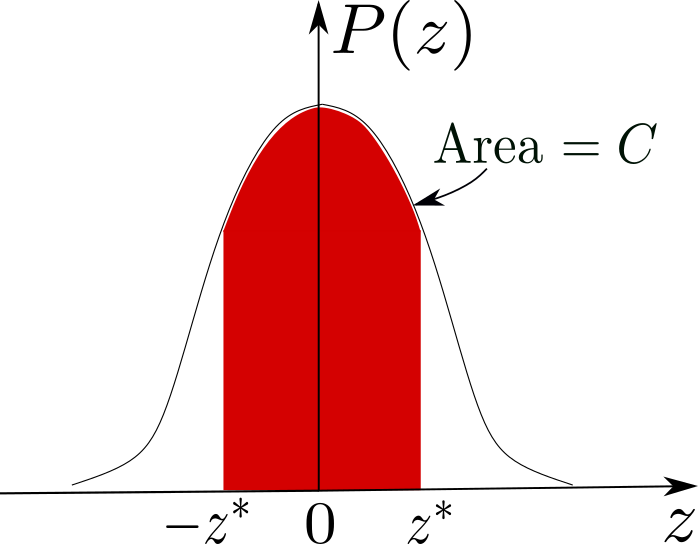
\includegraphics[width=2in]
{error-bars.png}
\caption{
Interpretation
of confidence level $C$.} 
\label{fig-error-bars}
\end{figure}

{\bf Confidence Level} $C$
and corresponding {\bf $z^*$ value}
(see Fig.\ref{fig-error-bars}):

\beq
C=\int_{-z^*}^{z^*} dz\;P(z) = 
\Phi(z^*)-\Phi(-z^*)
=
2\left(\Phi(z^*)-\frac{1}{2}\right)
\label{eq-conf-level1}
\eeq
Equivalent definition:

\beq
C=P\left(
\underbrace{
\frac{|\rvx-\mu|}{\frac{\sigma}{\sqrt{n}}}
}_{|z|}
<z^*\right)
\label{eq-conf-level2}
\eeq
For $C=95\%$,
$z^*=1.960\approx 2$.
For $C=99\%$, $z^*=2.576$.

Area of each tail 
in Fig.\ref{fig-error-bars} is
usually called $\alpha$:
\beq
C+2\alpha=1
\eeq  

Estimators\footnote{Don't 
confuse the sample index $\s$
with the standard deviation $\s$.} of 
mean $\mu$  and 
standard deviation $\sigma$
from measurements $x^\s$
of a sub-population $\Sigma_1$ of
size $n=|\Sigma_1|$:
\beq
\hat{\mu}=\ol{x}=\frac{1}{n}\sum_{\s \in\Sigma_1} x^\s
\eeq

\beq
\hat{\s}^2=
\frac{1}{n-1}
\sum_{\s\in \Sigma_1} (x^\s-\ol{x})^2
\eeq


We get
from Eq.(\ref{eq-conf-level2}),
the {\bf Error bars (aka confidence interval)}
and 
{\bf Error $E$ (aka margin of error)}:



\beq
\text{ estimate of $x$
with error bars} =
\ol{x} \pm 
\underbrace{
z^* \frac{\hat{\s}}{\sqrt{n}}}_{E}
\label{eq-err-bars}
\eeq

\beq
n= \left(
\frac{z^*\hat{\s}}{E}
\right)^2
\eeq

So far, we have assumed
that the sub-population (aka sample
population)
is normally distributed.
This might be false
for several reasons.
Some red flags: (1)
$n$ is too small (according to
a rule of thumb derived from
Central Limit Theorem, $n$
should be bigger than 30
to insure normality).
(2) Sub-population not truly random 
(i.i.d.) 
because was taken
without replacement.
In many cases,
especially
when $n<30$,
the Student's t-distribution
models the sub-population statistics
much
better than the Normal distribution.


The {\bf Student's t-distribution (SD)} $P_S(t;
\nu=n-1)$,
depends
on a parameter $\nu$
called the
number of
degrees of freedom.
In the case being considered here,
$\nu$ equals the 
sub-population size $n$
minus one.
When fitting
the data with
SD, variable
$t$ replaces
variable $z$,
and $P_S(t; \nu=n-1)$
replaces the Standard Normal distribution (SND) 
$\caln(z; \mu=0, \sigma=1)$.
SD is symmetric about
the origin like SND,
but its tails
are fatter.
When fitting the data with SD,
the $z^*$
value is replaced 
by a $t^*$ value.
Eq.(\ref{eq-conf-level1})
is replaced by


\beq
C=\int_{-t^*}^{t^*} dt\;P_S(t) = 
\Phi_S(t^*)-\Phi_S(-t^*)
=
2\left(\Phi_S(t^*)-\frac{1}{2}\right)
\label{eq-conf-level1-stu}
\;,
\eeq
where quantities subscripted by $S$
are for the SD,
Also, Eq.(\ref{eq-err-bars})
is replaced  by

\beq
\text{estimate of $x$
with error bars} =
\ol{x} \pm 
\underbrace{
t^* \frac{\hat{\s}}{\sqrt{n}}}_{E}
\;.
\eeq
Tables of $t^*(C,\nu=n-1)$
are available. Note 
that $t^*$
depends on both $C$ and $\nu$,
whereas $z^*(C)$
depends only on $C$.


\section{Short Summary of 
Boolean Algebra} 
See Ref.\cite{wiki-bool} for more info
about this topic.

Suppose $x, y, z\in \bool$. Define

\beq
x\text{ or }y=x\V y= x+y-xy
\;,
\eeq

\beq
x \text{ and }y=x\A y= xy
\;,
\eeq
and

\beq
\text{not }x=\ol{x}=1-x
\;,
\eeq
where we are using
normal addition and multiplication 
on the right hand sides.\footnote{Note the
difference between $\V$ and modulus
2 addition $\oplus$. 
For $\oplus$ (aka XOR): $x\oplus y=x+y-2xy$.}



\begin{table}[h!]
\centering
\begin{tabular}{|
>{\columncolor[HTML]{ECF4FF}}l |l|}
\hline
Associativity & \begin{tabular}[c]{@{}l@{}}$x \V (y \V z)=(x \V y) \V z$\\ $x \A (y \A z)=(x \A y) \A z$\end{tabular} \\ \hline
Commutativity & \begin{tabular}[c]{@{}l@{}}$x \V y=y \V x$\\ $x \A y=y \A x$\end{tabular} \\ \hline
Distributivity & \begin{tabular}[c]{@{}l@{}}$x \A (y \V z)=(x \A y) \V (x \A z)$\\ $x \V (y \A z)=(x \V y) \A (x \V z)$\end{tabular} \\ \hline
Identity & \begin{tabular}[c]{@{}l@{}}$x \V 0=x$\\ $x \A 1=x$\end{tabular} \\ \hline
Annihilator & \begin{tabular}[c]{@{}l@{}}$x \A 0=0$\\ $x \V 1= 1$\end{tabular} \\ \hline
Idempotence & \begin{tabular}[c]{@{}l@{}}$x \V x= x$\\ $x \A x= x$\end{tabular} \\ \hline
Absorption & \begin{tabular}[c]{@{}l@{}}$x \A (x \V y)= x$\\ $x \V (x \A y)= x$\end{tabular} \\ \hline
Complementation & \begin{tabular}[c]{@{}l@{}}$x \A \ol{x} = 0$\\ $x \V \ol{x}   = 1$\end{tabular} \\ \hline
Double negation & $\ol{(\ol{x})} = x$ \\ \hline
De Morgan Laws & \begin{tabular}[c]{@{}l@{}}$\ol{x} \A \ol{y} =\ol{(x \V y)}$\\ $\ol{x} \V \ol{y} = \ol{(x \A y)}$\end{tabular} \\ \hline
\end{tabular}
\caption{Boolean Algebra Identities}
\label{tab-bool-alg}
\end{table}

Actually, since
$x\A y=xy$, we can omit writing
the symbol $\A$. The symbol
$\A$ is useful to
exhibit the symmetry
of the identities, and
to remark
about
the analogous identities
for sets, where
$\A$ becomes intersection $\cap$
and $\V$ becomes union $\cup$. However,
for practical calculations,
$\A$ is an unnecessary nuisance.

Since $x\in \bool$,
\beq
P(\ol{x})=1-P(x)
\;.
\eeq

Clearly, from analyzing
the simple event space $(x,y)\in \bool^2$,
\beq
P(x\V y)= P(x) + P(y) - P(x\A y)
\;.
\eeq










